% file: 3-1-dp/rod-cutting-substructure.tex

\documentclass[tikz]{standalone}

\usetikzlibrary{positioning, calc, shapes.multipart, decorations.pathreplacing}
 
\begin{document}
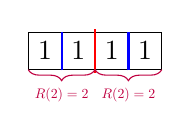
\begin{tikzpicture}[]
  \node (rod) [rectangle split, rectangle split parts = 4, draw, anchor = center, rectangle split horizontal]
    {$1$\nodepart{two}$1$\nodepart{three}$1$\nodepart{four}$1$};

  \draw [blue, thick] ($(rod.text split) + (0, -7pt)$) to ($(rod.text split) + (0, 7pt)$);
  \draw [red, thick] ($(rod.two split) + (0, -8pt)$) to ($(rod.two split) + (0, 8pt)$);
  \draw [blue, thick] ($(rod.three split) + (0, -7pt)$) to ($(rod.three split) + (0, 7pt)$);

  \draw [purple, decorate, decoration = {mirror, brace, amplitude = 4pt}, yshift = -10pt] 
  	(rod.south west) -- (rod.south) node [below = 5pt, scale = 0.5, midway] {$R(2) = 2$};
  \draw [purple, decorate, decoration = {mirror, brace, amplitude = 4pt}, yshift = -10pt] 
  	(rod.south) -- (rod.south east) node [below = 5pt, scale = 0.5, midway] {$R(2) = 2$};
\end{tikzpicture}
\end{document}
